\documentclass[conference]{IEEEtran}
\IEEEoverridecommandlockouts
% The preceding line is only needed to identify funding in the first footnote. If that is unneeded, please comment it out.
\usepackage{cite}
\usepackage{amsmath,amssymb,amsfonts}
\usepackage{algorithmic}
\usepackage{graphicx}
\usepackage{textcomp}
\usepackage{xcolor}
\def\BibTeX{{\rm B\kern-.05em{\sc i\kern-.025em b}\kern-.08em
    T\kern-.1667em\lower.7ex\hbox{E}\kern-.125emX}}
\begin{document}

\title{Automatic Play Gaming With Deep Learning\\
%{\footnotesize \textsuperscript{*}Note: Sub-titles are not captured in Xplore and
%should not be used}
}

\author{\IEEEauthorblockN{Miguel Antonio Rodriguez Delgado}
\IEEEauthorblockA{\textit{Electronic Engineering} \\
\textit{\textbf{Hamm-Lippstadt University of Applied Sciences}}\\
Dortmund, Germany \\
miguel-antonio.rodriguez-delgado@stud.hshl.de}
}

\maketitle

\begin{abstract}

Deep learning techniques are growing in all fields, and game playing in not an exception. With this paper we review how different deep learning methods to understand how the can be used in gaming environments. Along this paper we will show how deep learning can be applied for a real world example, focusing in the development of the well known Tic-tac-toe game. We also share the results of the comparison using deep learning techniques against coding the the same game in a classical way.


\end{abstract}

\begin{IEEEkeywords}
Deep learning, Automatic Play Gaming, Tic-tac-toe, Minimax, Neural-networks.
\end{IEEEkeywords}

\section{Introduction}\label{sec:intro}

Video games industry is becoming an important part on people's life, not only by offering entertainment, but also by offering sense of belonging and interconnecting people \cite{niche}. Reports of the Entertainment Software Association (ESA) on 2020 showed that nowadays, and boosted by the corona-virus lockdown  not only young males, but also women, adults and even retired people is attracted by this industry \cite{niche}.

Deep learning algorithms and Artificial Intelligence (AI) have been used in may fields, including the video game industry since 1971, starting with Computer Space and Pong on the Atari 2600 \cite{atari}.

Artificial Intelligence is defined the study of "Intelligent Agents", as any device that can perceive its environment and based on it attempt to take actions to succeed in a goal by maximizing its chances of success \cite{ai}. Machine learning and deep learning algorithms are the tools used to generate these so called intelligent agents \cite{ai}.


\section{Artificial Intelligence On Games}

As described on \ref{sec:intro}, AI has been present in games since the earlies seventies, 
\cite{sony}. However, in the 1957  a team at Carnegie Mellon University predicted that in 1967 a computer would have been capable of defeating a chess world champion \cite{euristic}, but they did not anticipate the hight complexity to predict the correct order of movements required for this task. But at the end of the decade of seventies, a computer defeated for the first time a world champion level chess player \cite{bad}.

In the same way, Artificial Intelligence has been used to defeat humans in other games, such as Mahjong and Go \cite{sony}. These kind of games required a lot of computation and learning algorithm, but they have the possibility to take the time to perform all the necessary calculations. But more advance games, such as Sony's Gran Turismo, have an increased difficulty to master the correct algorithm to drive a race car since many decisions have to be made in real time \cite{sony}.

\subsection{Chess}

The British mathematician and computer scientist Alan Turing was one of the scientist that developed the first algorithm for playing chess. The design of the algorithm was made to be run on a computer that did not exist at that time \cite{how}.

On 1951 Alan Turing with David Gawen Champernowne deigned a heuristic algorithm and they try to run in on a 1951 Ferranti Mark 1 computer, but due to the limitations of the computational power of the machine the task was impossible for the computer \cite{how}.

Each position on a chess game can be represented as outcome of all the previous positions and moves. For this reason, a chess program do not only need to take into account the current move but the previous and even most important, the possible next moves \cite{how}. In Figure \ref{chess:tree} we can see a tree of how each move can generate a limited number of moves, and how the tree grow deeper after every move, so the chess program can select the best next move \cite{how}

\begin{figure}[h]
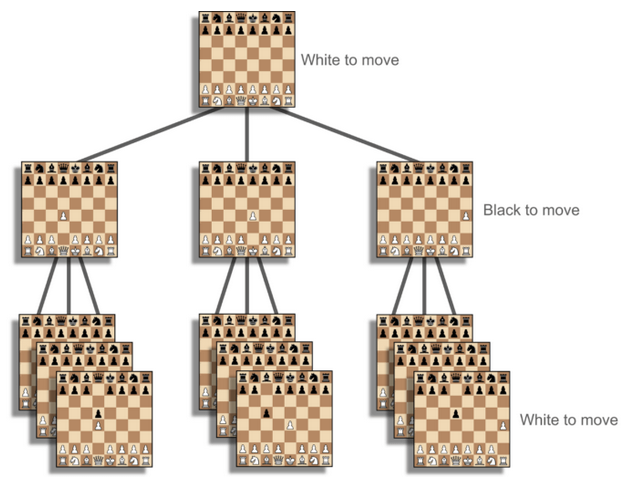
\includegraphics[scale=0.52]{img/tree}
\caption{Searching tree on a chess game \cite{how}}
\label{chess:tree}
\end{figure}

According to Claude Shannon there are two main ways of searching on a chess program, brute-force and selective searches. The first one takes a look at every movement on the board but with a fixed depth of movements, while the second one search for the best candidates going through all the moves and ignore the other branches \cite{how}

Some of the most important algorithms include Chess Challenger, Chessmaster, IBM’s Deep Blue and Alpha-Beta Pruning, but since they will be let out of the scope of this research to focus on Deep Mind, which uses \textit{Residual Policy and Value Networks} and \textit{Reinforcement Learning}


\ref{chess:reinforcement}

\begin{figure}[h]
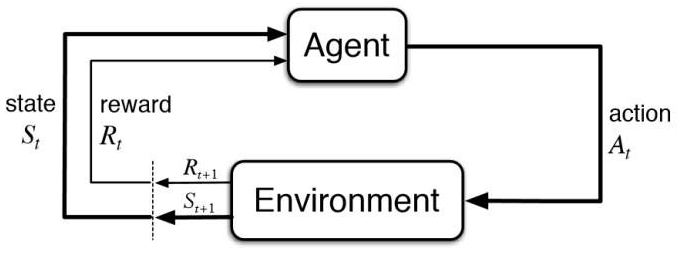
\includegraphics[scale=0.52]{img/deepchess}
\caption{Reinforcement learning on Deep Main algorithm \cite{how}}
\label{chess:reinforcement}
\end{figure}





\subsection{Racing games}

Since the introduction of deep learning for racing games, reinforcement learning and supervised learning have been the two principal ways to train a network to learn how to drive a car \cite{racingpdf}.

For the reinforcement learning process, the computer learns on its own by trial and error \cite{racingpdf}. Consequently, it is not required to have a big set of data before starting with the training \cite{racingpdf}. The most important attributes to train a network with reinforcement learning are an agent and an environment \cite{racingpdf}.

Gran Turismo, a racing simulation video game, made its debut in 1997 and has sold over 80 million units.
According to Sony, it took about 20 PlayStations running simultaneously during 12 days to train Sophy, the Gran Turismo artificial intelligence 


\section{Drawbacks}

The introduction of artificial intelligence and deep learning algorithms do not only offer advantages in the different fields that we have talk about in the previous sections, but it also brings different risks. Since the focus of study of this paper is gaming, an example on how AI can represent a risk in the development of a chess software that can identify unique styles of playing and it is able to point out with no previous information, who it is playing with, what represent a serious privacy risk \cite{unmask}.

\section{Case Of Study - Tic-Tack-Toe}



Neural networks, genetic programming, computer vision, heuristic search, knowledge representation and reasoning, Bayes networks, planning, and language understanding are each revealed through the growing capabilities of these agents.



\begin{thebibliography}{00}

\bibitem{niche} Lugris, M. (2020, July 25). New ESA Report Shows Gaming Is No Longer A Niche Market. TheGamer. https://www.thegamer.com/esa-gaming-niche-popular-die-mad-gamers/

\bibitem{atari} Skinner, G.,  $\&$ Walmsley, T. (2019, February). Artificial intelligence and deep learning in video games a brief review. In 2019 IEEE 4th International Conference on Computer and Communication Systems (ICCCS) (pp. 404-408). IEEE.

\bibitem{ai} Ongsulee, P. (2017, November). Artificial intelligence, machine learning and deep learning. In 2017 15th international conference on ICT and knowledge engineering (ICT$\&$KE) (pp. 1-6). IEEE.

\bibitem{euristic} A. Newell and H. Simon, “Heuristic Problem-Solving: The Next Advance in Operation Research,” Operations Research, Vol. 6, No. 6, 1958. 

\bibitem{bad} Hapgood, Fred. "Computer chess bad-human chess worse". New Scientist. pp. 827–830. (23–30 December 1982) Retrieved 22 January 2015.

\bibitem {how}How does AI play chess? (2022, September). Baeldung. https://www.baeldung.com/cs/ai-chess

\bibitem{sony} Mukherjee, S. (2022, February 9). Sony’s new AI beats humans in Gran Turismo racing game. Reuters. https://www.reuters.com/technology/sonys-new-ai-beats-humans-gran-turismo-racing-game-2022-02-09/

\bibitem{racing} Lecchi, S. (2009, September). Artificial intelligence in racing games. In 2009 IEEE Symposium on Computational Intelligence and Games (pp. 1-1). IEEE.

\bibitem{racingpdf} Teigar, H., Storožev, M., $\&$ Saks, J. (2017). 2D Racing game using reinforcement learning and supervised learning.

\bibitem{automated} Hutter, F., Kotthoff, L., $\&$ Vanschoren, J. (2019). Automated machine learning: methods, systems, challenges (p. 219). Springer Nature.

\bibitem{wild} Stadelmann, T., Amirian, M., Arabaci, I., Arnold, M., Duivesteijn, G. F., Elezi, I., $\&$ Tuggener, L. (2018, September). Deep learning in the wild. In IAPR Workshop on Artificial Neural Networks in Pattern Recognition (pp. 17-38). Springer, Cham.

\bibitem{unmask} Hutson, M. (2022). Artificial intelligence unmasks anonymous chess players. Science, 129, 129.


\end{thebibliography}
\end{document}
